\apendice{Documentación técnica de programación}

\section{Introducción}
En este anexo se va a describir con detalle la documentación técnica de programación. Se describirá la estructura de directorios que posee, la instalación del propio entorno de desarrollo, cómo llevar a cabo su compilación, instalación y ejecución; además de las pruebas que se han realizado.

Se debe recordar que el proyecto se encuentra dividido en dos repositorios diferenciados, UBUMLaaS e IS-SSL\footnote{Biblioteca de algoritmos de selección de instancias y aprendizaje semi-supervisado programado.}; es por ello que, se dividirá en dos secciones respectivamente, y tantas subsecciones como son necesarias para cada uno de ellos.

Ambos repositorios son consultables desde:
\begin{itemize}
\tightlist
\item \textbf{\texttt{UBUMLaaS}.}~\url{https://github.com/dpr1005/UBUMLaaS}
\item \textbf{\texttt{IS-SSL}.}~\url{https://github.com/dpr1005/Semisupervised-learning-and-instance-selection-methods} 
\end{itemize}

\section{UBUMLaaS}

\subsection{Estructura de directorios}
La estructura del repositorio es la siguiente:
\begin{itemize}
\tightlist
\item \texttt{/}: raíz del proyecto, aquí se encuentra el README, la licencia, los ficheros de configuración de las pruebas de integración y despliegue continuo (CI-CD), junto con los ficheros de requisitos para \texttt{conda} y \texttt{pyenv}. 
\item \texttt{/lib/}: librerías utilizadas por el sistema.
\item \texttt{/lib/is\_ssl}: librería propia de métodos de selección de instancias y aprendizaje semi-supervisado.
\item \texttt{/lib/scikit\_ml\_learn\_data/meka/meka-release-1.9.2/}: librería \texttt{Meka} en su versión 1.9.2.
\item \texttt{/lib/skmultilearn/}: librería \texttt{scikit-multilearn}.
\item \texttt{/lib/unofficial\_weka\_packages/}: algoritmos de ADMIRABLE.
\item \texttt{/lib/wekafiles/}: algoritmos concretos de \texttt{weka}.
\item \texttt{/test/*}: ficheros de prueba CI-CD.
\item \texttt{/ubumlaas/}: directorio principal de la plataforma.
\item \texttt{/ubumlaas/admin/}: contiene toda la parte de \textit{backend} de administración.
\item \texttt{/ubumlaas/core/}: contiene el \textit{backend} de las vistas de índice y acerca de.
\item \texttt{/ubumlaas/default\_datasets/}: conjuntos de datos por defecto que se añaden a los nuevos usuarios.
\item \texttt{/ubumlaas/error\_pages/}: contiene el \textit{backend} de las vistas de error.
\item \texttt{/ubumlaas/experiments/}: contiene el \textit{backend} para la realización de experimentos.
\item \texttt{/ubumlaas/experiments/algorithm/}: contiene las métricas para el análisis del modelo entrenado.
\item \texttt{/ubumlaas/experiments/execute\_algorithm/}: contiene opciones de ejecución para cada librería.
\item \texttt{/ubumlaas/experiments/views/}: control de las vistas relacionadas con los experimentos.
\item \texttt{/ubumlaas/jobs/}: descripción de \textit{RQ Worker Builder}.
\item \texttt{/ubumlaas/static/}: contiene los ficheros estáticos de la plataforma.
\item \texttt{/ubumlaas/static/avatars/}: contiene las imágenes de perfil de cada usuario.
\item \texttt{/ubumlaas/static/css/}: contiene el código \texttt{CSS} del \textit{frontend}.
\item \texttt{/ubumlaas/static/img/}: contiene las imágenes que aparecen en la pltaforma.
\item \texttt{/ubumlaas/static/js/}: contiene el código \texttt{JavaScript} del \textit{frontend}.
\item \texttt{/ubumlaas/templates/}: ficheros \texttt{HTML}.
\item \texttt{/ubumlaas/templates/admin/}: ficheros web de administración.
\item \texttt{/ubumlaas/templates/blocks/}: ficheros web de bloques que se añaden sobre otros documentos web.
\item \texttt{/ubumlaas/templates/error\_pages/}: ficheros web de errores (403, 404, \dots)
\item \texttt{/ubumlaas/templates/modals/}: ficheros para la representación de modales.
\item \texttt{/ubumlaas/users/}: contiene el \textit{backend} de las actividades relacionadas con el usuario.
\item \texttt{/ubumlaas/weka/}: contiene los ficheros de configuración de \texttt{Weka} y su \texttt{VM}.

\end{itemize}

\subsection{Manual del programador}
En esta subsección se describen todos aquellos recursos utilizados por el equipo de desarrollo para, valga la redundancia, desarrollar el proyecto. De tal forma que un futuro desarrollador/mantenedor del proyecto no tenga inconvenientes a la hora de retomar el proyecto y conocerlo.

\subsubsection{Entorno de desarrollo}
Para poder continuar con el desarrollo del proyecto, se requiere tener instalado el siguiente \textit{software} en el equipo:
\begin{itemize}
\tightlist
\item Python 3.7+.
\item Bibliotecas Python.
\item Git
\item VSCode
\end{itemize}

En los siguientes apartados se detalla la instalación de cada uno de los componentes anteriormente citados.

\subsubsection{Python 3.7+}
Al comienzo del proyecto, muchas de sus funcionalidades eran compatibles con Python 2, pero el nuevo desarrollo ha utilizado indistintamente métodos existentes en versiones anteriores de Python y algunos que se han introducido a partir de la version 3.7, disponible desde~\cite{pythonGetIt}. Es importante que los binarios se encuentren en el \texttt{path} del sistema para que no de problemas de ejecución.

\subsubsection{Bibliotecas Python}
A continuación (ver Tabla~\ref{tab:bibliotecas-python-ubumlaas}), se van a detallar uno de los puntos más importantes para poder <<hacer funcionar>> el proyecto, puesto que se van a necesitar versiones concretas de determinadas librerías para que todo se integre correctamente con todo y se pueda ver y utilizar como un sistema homogéneo.

\begin{table}[p]
\centering
\begin{tabular}{lcl}
	\toprule
	\textbf{Biblioteca} & \textbf{Versión} & \textbf{Descripción}\\
	\midrule
	\rowcolor[HTML]{EFEFEF} 
	\texttt{email-validator} & 1.1.1 & Validar direcciones de correo electrónico.\\
	\texttt{flask} & 1.1.1 & Web \textit{framework}.\\ \rowcolor[HTML]{EFEFEF}
	\texttt{flask-login} & 0.4.1 & Control usuarios y sesiones en Flask.\\
	\texttt{flask-mail} & 0.9.1 & Envío de \textit{emails} con Flask.\\ \rowcolor[HTML]{EFEFEF}
	\texttt{flask-migrate} & 2.5.2 & Migrar SQLAchemy DB a Flask.\\
	\texttt{flask-redis} & 0.4.0 & Soporte a Redis en Flask.\\ \rowcolor[HTML]{EFEFEF}
	\texttt{flask-sqlalchemy} & 2.4.0 & Soporte a SQLAchemy en Flask.\\
	\texttt{flask-wtf} & 0.14.2 & Render, validar y CSRF formularios.\\ \rowcolor[HTML]{EFEFEF}
	\texttt{future} & 0.16.0 & Soporte a Python 2 y 3.\\ 
	\texttt{geopy} & 2.2.0 & Geocodificación.\\ \rowcolor[HTML]{EFEFEF}
	\texttt{glances} & 3.2.4.2 & Monitorización del sistema.\\ 
	\texttt{imbalanced-learn} & 0.5.0 & ML con datos desbalanceados.\\ \rowcolor[HTML]{EFEFEF}
	\texttt{itsdangerous} & 1.1.0 & Paso de datos en entornos no seguros.\\
	\texttt{liac-arff} & 2.2.1 & Escritura y lectura de ficheros ARFF.\\ \rowcolor[HTML]{EFEFEF}
	\texttt{numpy} & 1.22.3 & Computación de \textit{arrays}.\\
	\texttt{pandas} & 0.25.1 & Estructuras de datos.\\ \rowcolor[HTML]{EFEFEF}
	\texttt{psutil} & 5.9.0 & Procesar y monitorizar sistemas.\\
	\texttt{pycountry} & 22.3.5 & Datos de países.\\ \rowcolor[HTML]{EFEFEF}
	\texttt{pytest} & 5.2.1 & Pruebas en Python.\\
	\texttt{python-weka-wrapper3} & 0.1.7 & \textit{Wrapper} para Weka.\\ \rowcolor[HTML]{EFEFEF}
	\texttt{requests} & 2.22.0 & \textit{Requests} para humanos.\\
	\texttt{rq} & 1.1.0 & Crear y procesar trabajos <<de fondo>>.\\ \rowcolor[HTML]{EFEFEF}
	\texttt{scikit-learn} & 0.24 & Módulos de minería de datos y ML.\\ 
	\texttt{selenium} & 3.141.0 & Auto interacción con navegador web.\\ \rowcolor[HTML]{EFEFEF}
	\texttt{urllib3} & 1.25.6 & Conexiones HTTP seguras.\\
	\texttt{werkzeug} & 0.15.6 & Biblioteca de aplicaciones web WSGI.\footnote{\textit{Web Server Gateway Interface.}. Es una especificación que describe cómo un servidor web se comunica con las aplicaciones web, y cómo las aplicaciones web pueden encadenarse para procesar una solicitud.}\\ \rowcolor[HTML]{EFEFEF}
	\texttt{whichcraft} & 0.4.1 & Funcionalidad \textit{shutil.which}. \\
	\bottomrule
\end{tabular}
\caption{Bibliotecas utilizadas por UBUMLaaS y sus versiones.}\label{tab:bibliotecas-python-ubumlaas}
\end{table}

Las versiones indicadas en la tabla~\ref{tab:bibliotecas-python-ubumlaas} son las que se han utilizado para el desarrollo del proyecto, se pueden actualizar a versiones futuras, siempre y cuando sean compatibles entre sí.

\subsection{Compilación, instalación y ejecución del proyecto}
En esta subsección se va a detallar el proceso a seguir para poder hacer uso del proyecto en local, modificarlo y/o utilizarlo. La forma de desarrollo del proyecto no ha sido estrictamente en local, sino que el proyecto se encontraba alojado en un equipo servidor y mediante SSH\footnote{\textit{Suite} de protocolos los cuales especifican estándares para operar los servicios de red de forma segura entre anfitriones para los que no existe una relación de confianza a través de redes no seguras. Las comunicaciones entre pares se encuentran encriptadas.} se realizaba la conexión y posterior edición de los ficheros.

\subsubsection{Adquisición del código fuente}
Lo primero que se necesita es obtener el código en el equipo, para ello podemos seguir una de las siguientes aproximaciones:
\begin{itemize}
\item Mediante el uso de la terminal.
\begin{enumerate}
\tightlist
\item Apertura de la terminal.
\item Desplazarse al directorio en donde se desee clonar el repositorio (usando \texttt{cd} en Unix o \texttt{dir} en Windows).
\item Hacer uso del siguiente comando:\\
\texttt{git clone https://github.com/dpr1005/UBUMLaaS.git}
\item Se dispone de una copia idéntica a la alojada en el repositorio de \texttt{GitHub}.
\end{enumerate}

\item Descarga desde el navegador.
\begin{itemize}
\tightlist
\item Apertura del navegador preferido.
\item Introducir en la barra de búsqueda la siguiente dirección:\\
\texttt{https://github.com/dpr1005/UBUMLaaS/archive/refs/\\heads/master.zip}
\item Aceptar la descarga en caso de tener habilitada la comprobación.
\item Navegar con el Explorador de archivos del sistema hasta el directorio de descarga.
\end{itemize}

\item Uso de \texttt{GitKraken}.
\begin{itemize}
\tightlist
\item Apertura de la aplicación.
\item Hacer \textit{click} en \textit{Clone a repo}.
\item En \textit{Repository Management} $\rightarrow$ \textit{Clone} $\rightarrow$ \textit{Clone with URL}: 
\begin{itemize}
\item Indicar la ruta local en la que nos interesa que se clone el repositorio.
\item En URL introducir:\\
\texttt{git clone https://github.com/dpr1005/UBUMLaaS.git}
\end{itemize}
\item Hacer \textit{click} en \textit{Clone the repo!}.
\end{itemize}
\end{itemize}

\subsubsection{Importar el proyecto en Visual Studio Code}
Se diferencian dos aproximaciones, local o como se ha operado, conexión mediante SSH.

\begin{itemize}
\item Importar el proyecto en la propia máquina donde se va a desplegar y será en ella en la que se edite.
\begin{enumerate}
\item Apertura de \texttt{Visual Studio Code}.
\item Hacer \textit{click} en Abrir.
\item Seleccionar el directorio raíz donde lo hayamos alojado.
\end{enumerate}
\item Importar el proyecto en una máquina y editarlo desde otra.
\begin{enumerate}
\item Seguir los pasos de la adquisición del código en la máquina en la que se va a alojar el código. En el equipo local no va a estar.
\item Apertura de \texttt{Visual Studio Code}
\item Navegar a las Extensiones e instalar \texttt{Remote - SSH}, disponible desde~\cite{VSCode-Remote-SSH}.
\item Instalar un cliente SSH compatible con \texttt{OpenSSH}. Ver guía~\cite{Remote-Development-Tricks-Tips}.
\item Con todo instalado, se realiza la conexión a la máquina remota.
\begin{enumerate}
\item Presionar \texttt{F1} y correr el comando: \texttt{Remote-SSH: Open SSH Host...}
\item Introducir el usuario y el \texttt{host/IP} en el formato:\\
\texttt{user@host-o-ip} ó \texttt{user@domain@host-o-ip}
\item En caso de que se solicite, introducir la contraseña, pero se recomienda configurar el uso de llaves SSH, ver guía~\cite{Remote-Development-Tricks-Tips}.
\item Después de la conexión usar Archivo $\rightarrow$ Abrir carpeta, para abrir el directorio donde se encuentra el proyecto en la máquina remota.
\end{enumerate}
\item Todos los cambios que se realicen, se harán sobre el código en la máquina remota, la máquina local no hará más que el efecto de editor.
\end{enumerate}
\end{itemize}

\subsubsection{Crear entorno virtual de trabajo}
Para poder trabajar con este proyecto (independientemente de si es para desarrollo o producción) hacen falta una serie de bibliotecas concretas de Python, las cuales, como es lógico, deben estar en la máquina en la que se va a ejecutar; dicho con otras palabras, en la que está el código. El proyecto está preparado para crear un entorno de \texttt{Conda} propio, de forma que no interfiera con otros proyectos y sea más sencillo de mantener y actualizar.

Se recomienda que los binarios de anaconda o miniconda estén configurados en el \texttt{path} del sistema para poder utilizar el comando \texttt{conda} desde la línea de comandos.

El proceso de creación del entrono virtual con \texttt{Conda} es el siguiente:
\begin{enumerate}
\tightlist
\item Apertura de la terminal.
\item Navegar hasta la raíz del proyecto.
\item Crear el entorno con:\\
\texttt{conda env create -f UBUMLaaS\_env.yml}
\item Cuando se desee utilizar se debe activar:\\
\texttt{conda activate UBUMLaaS}
\end{enumerate}

También se puede utilizar el procedimiento habitual para importar las bibliotecas al actual \texttt{venv} de la sesión de la terminal, pero se desaconseja su uso ya que un entorno <<genérico>> antes o después se actualizará por otros proyectos, pudiendo generar incompatibilidades con el proyecto UBUMLaaS.

\subsubsection{Instalación en Linux}
Con los anteriores pasos realizados, la importación del proyecto y la activación del entorno virtual, se deben modificar una serie de ficheros con el fin de habilitar todas las funcionalidades que ofrece el proyecto. 

Se deben seguir los siguientes pasos:
\begin{enumerate}
\item Modificar \texttt{env\_variables.sh} con los valores correctos para cada uno de los campos:
\begin{lstlisting}[language=bash]
export SECRET_KEY=<app secret key>
export EMAIL_AC=<email>
export EMAIL_PASS=<email-password>
export EMAIL_URL=<email-url>
export FLASK_ENV=development #development or production
LIBFOLDER=/absolute/path/to/UBUMLaaS
\end{lstlisting}
\item Dentro del entorno virtual de UBUMLaaS en \texttt{Conda}, se debe ejecutar el siguiente comando para permitir la importación de las variables anteriormente declaradas al entorno virtual.\\
\texttt{source env\_vars\_to\_conda.sh}
\item Creación de la base de datos.\\
\texttt{mv data\_base.sqlite ubumlaas/data.sqlite}\\
* En caso de poseer una base de datos con la configuración correcta, se puede poner en \texttt{./ubumlaas/} bajo el nombre de \texttt{data.sqlite}.
\item En caso de no tener instalado y configurado \texttt{Redis-Server}, ejecutar:
\begin{lstlisting}[language=bash]
sudo apt install redis-server
sudo service redis-server start
sudo systemctl enable redis-server
\end{lstlisting}
\end{enumerate}

\subsubsection{Uso del proyecto}
Lo primero de todo para poder tener el producto trabajando, es desplegarlo, para ello es requisito haber completado todos los pasos previos de esta sección. Activar el entorno virtual de \texttt{Conda}, ejecutar el lanzador, y ya está en ejecución.
\begin{lstlisting}[language=bash]
conda activate UBUMLaaS
./run.sh
\end{lstlisting}
\textbf{Nota.} Es importante asegurarnos que todos los ficheros de las librerías y el lanzador del proyecto poseen permisos de ejecución necesarios (en instalaciones <<por defecto>> de Debian, CentOS, SUSE, no debería de ser necesario más que dar permisos de ejecución al lanzador).

El usuario administrador por defecto es \texttt{Admin@AdminUBUMLaaS.es} y su contraseña es \texttt{admin4123!UBUMLaaS}.

\subsection{Integración Continua}
Con el objetivo de obtener como producto final un \textit{software} de calidad, se han desarrollado una serie de pruebas de integración continua, las cuales se comprueban y analiza su resultado en cada \textit{commit} y/o \textit{pull request.}

Se han utilizado principalmente tres herramientas \textit{cloud} para medir los principios de calidad del \textit{software}.

\subsubsection{Codacy}
Herramienta la cual proporciona soporte a análisis automático del código fuente e identifica los problemas a medida que avanza. Su versatilidad permite desarrollar \textit{software} de manera eficiente, reduciendo el número de \textit{bugs} que se <<dejan para resolver>>. 

A través del análisis de código estático, notifica problemas de seguridad, cobertura del código, así como la duplicación y la complejidad de cada fichero en cada \textit{commit} y \textit{pull request}.

\imagenRuta{../img/anexos/manual-programador/Codacy-UBUMLaaS}{Codacy.}{Codacy-UBUMLaaS}

\subsubsection{Sonar Cloud}
Herramienta \textit{open source} la cual permite hacer un análisis estático del código de un proyecto, entre sus fortalezas destaca su potente capacidad de ser parametrizada, entre las acciones que realiza por defecto encontramos la detección de malas prácticas, errores de código, así como problemas de seguridad que en el pasado se han visto relacionadas con alguna CVE\footnote{\textit{Common Vulnerabilities and Exposures}, lista de fallos \textit{software} (y \textit{hardware}) que en el pasado se han utilizado para ganar ventaja de alguna manera.}.

A pesar de que sea un proyecto \textit{open source} no es gratuita, y como todas las herramientas de estas características incluye una versión \textit{community} (gratuita) para aquellos proyectos que sean \textit{open source}.

\imagenRuta{../img/anexos/manual-programador/SonarCloud-UBUMLaaS}{SonarCloud.}{SonarCloud-UBUMLaaS}

\subsubsection{Travis-CI}
Herramienta \textit{cloud} desarrollada para la realización de pruebas de integración continua sobre proyectos alojados en GitHub (con soporte beta para BitBucket, Gitlab y Assembla). Permite realizar un \textit{build} del proyecto y ejecutar sobre ella una batería de pruebas de manera automática cada vez que se realiza un \textit{commit} y/o \textit{pull request}, permitiendo pruebas concurrentes, incluso sobre diferentes sistemas operativos (Linux, Windows, macOS y FreeBSD). 

Con el proyecto configurado en \texttt{Travis-CI} se debe configurar un fichero \texttt{YAML} y debe de estar en el directorio raíz, será a partir del cual se ejecuten las pruebas.

El fichero se encuentra dividido en:
\begin{itemize}
\tightlist
\item \texttt{os:} sistema/s operativo/s sobre el cuál se va/n a realizar las pruebas.
\item \texttt{dist:} distribución a utilizar.
\item \texttt{language:} lenguaje de programación del proyecto.
\item \texttt{python:} especificación de la versión de Python que necesita.
\item \texttt{node\_js:} especificación de la versión de Node JS que necesita.
\item \texttt{jdk:} especificación de la versión de JDK necesaria.
\item \texttt{jobs:} parametrización de los trabajos que se van a ejecutar.
\item \texttt{git:} profundidad del árbol de \texttt{git} que deseamos utilizar.
\item \texttt{addons:} \textit{software} <<extra>> que se necesiten para las pruebas.
\item \texttt{services:} especificación de los servicios que se van a utilizar.
\item \texttt{before\_install:} definición de comandos a ejecutar antes de los incluidos en la sección \texttt{install}.
\item \texttt{install:} definición de comandos de instalación de dependencias.
\item \texttt{before\_script:} configuración de dependencias antes de ejecutar la sección \texttt{script}.
\item \texttt{script:} pruebas a realizar.
\end{itemize}

Los \textit{logs} son públicos y consultables desde~\cite{Travis-CI-LOG-UBUMLaaS}.

\imagenRuta{../img/anexos/manual-programador/Travis-CI-UBUMLaaS}{Travis-CI.}{Travis-CI-UBUMLaaS}

\subsection{Pruebas del sistema}
Las pruebas del sistema se encuentran dentro de los trabajos futuros que debe seguir la aplicación.

Tal y como se ha descrito, \texttt{UBUMLaaS} es un \textit{software} que ha sufrido un cambio de diseño de grandes dimensiones, por lo que las pruebas de integración continua previas que existían han dejado de ser funcionales. La problemática que surge con las existentes es que no eran pruebas sobre el \textit{backend} de la aplicación, sino la interacción del usuario (mediante el uso de \textit{Selenium}) con el \textit{frontend}. 

Es por ello que, al haberse hecho <<de cero>> toda la interfaz de la aplicación web, literalmente, no existe ninguna referencia de las antiguas que las pruebas existentes puedan reutilizar. 

Debido a esta problemática, y con el fin de obtener un sistema estable, se ha seleccionado a un grupo de personas de edades comprendidas entre 18 y 55 años, profesionales de mecánica y electrónica, medicina, informática y estudiantes del grado de otras universidades españolas; con el fin de que dado un \href{https://github.com/dpr1005/Semisupervised-learning-and-instance-selection-methods/blob/917d49bcc9d7f1a4825225414b246023bfa2ea7b/docs/misc/survey_steps.pdf}{documento} relativamente sencillo, puedan hacer uso de todo el sistema, y sean estos los que reporten en un \href{https://forms.gle/eZUWmT5GNahqYVVa6}{formulario de \texttt{Google}} sus impresiones y resultados. Está preparado para que se vaya leyendo el documento, probando la aplicación y posteriormente rellenando el formulario, de forma que todo sea un proceso auto-guiado.

Gracias a estas respuestas, se han podido encontrar \textit{bugs} existentes en la aplicación que no permitían trabajar correctamente con ella. El más importante de todo y el cual posee su propia \href{https://github.com/dpr1005/UBUMLaaS/issues/101}{\textit{issue}}, es el desfase existente entre los algoritmos de \texttt{Scikit-Learn} de la versión 0.21 (la utilizada previamente) y la actual, la 0.24. Numerosos algoritmos han sido modificados en su parametrización y por ende en \texttt{UBUMLaaS} no se podían utilizar.

Durante algunos meses de desarrollo del proyecto \texttt{Travis-CI} funcionó correctamente pero la propia herramienta sufrió una actualización a finales de marzo y dejó de ser funcional, resultando en numerosos \textit{commits} marcados como erróneos, pero tal y como se aprecia en los propios \textit{logs} de Travis, nunca se llegó a testar el código, sino que en la configuración de la máquina remota <<rompía>>.

\clearpage
\section{IS-SSL}

\subsection{Estructura de directorios}
La estructura del repositorio es la siguiente:
\begin{itemize}
\item \texttt{/}: raíz del proyecto, aquí se encuentra el README, la licencia, los ficheros de configuración de PIP, los ficheros de configuración de las pruebas de integración y despliegue continuo (CI-CD); y, el fichero de requisitos.
\item \texttt{/datasets/*}: conjuntos de datasets en formatos \texttt{csv} y \texttt{arff}, normalizados y no normalizados.
\item \texttt{/docs/}: documentación del proyecto.
\item \texttt{/docs/img/}: imágenes utilizadas en la documentación.
\item \texttt{/docs/img/anexos/*}: imágenes utilizadas en los anexos.
\item \texttt{/docs/img/draws/}: diagramas en su formato original.
\item \texttt{/docs/img/memoria/*}: imágenes utilizadas en la memoria.
\item \texttt{/hypothesis/*}: primera aproximación a la investigación realizada.
\item \texttt{/implementation\_tests/}: conjunto de pruebas de validación sobre los algoritmos implementados.
\item \texttt{/instance\_selection/}: algoritmos implementados de selección de instancias.
\item \texttt{/instance\_selection/utils/}: métodos de apoyo comunes a los algoritmos de selección de instancias.
\item \texttt{/misc/}: contiene archivos varios de formato para el repositorio (cabeceras, logos, etc.).
\item \texttt{/semisupervised/}: algoritmos implementados de aprendizaje semi-supervisado.
\item \texttt{/semisupervised/utils/}: métodos de apoyo comunes a los algoritmos de aprendizaje semi-supervisado.
\item \texttt{/utils/}: diferentes clases y métodos de apoyo comunes tanto a selección de instancias como a semi-supervisado.
\end{itemize}

\subsection{Manual del programador}
En esta subsección se describen todos aquellos métodos seguidos por el equipo de desarrollo para, valga la redundancia, desarrollar el proyecto. De tal forma que un futuro desarrollador no tenga inconvenientes a la hora de retomar el proyecto.

\subsubsection{Entorno de desarrollo}
Para poder continuar con el desarrollo del proyecto, se requiere tener instalado el siguiente \textit{software} en el equipo:
\begin{itemize}
\tightlist
\item Python 3.7+.
\item Bibliotecas Python.
\item Git
\item VSCode/PyCharm/\dots.
\end{itemize}

En los siguientes apartados se detalla la instalación de cada uno de los componentes anteriormente citados.

\subsubsection{Python 3.7+}
El desarrollo se ha realizado siguiendo las últimas formas de programación disponibles a partir de la versión 3.7 de Python. El desarrollo se comenzó después de que se dejara de mantener Python 2, por lo que se trabajó desde el inicio con versiones de Python 3. Se puede obtener la última versión disponible de Python desde~\cite{pythonGetIt}. Es importante que el desarrollador se asegure que los binarios han sido añadidos al \texttt{path} del sistema que esté utilizando.

\subsubsection{Bibliotecas Python}
Esta sección es la más importante de todas junto con la anterior, debido a que el proyecto depende de (está construido utilizando) bibliotecas de $3^{os}$. Y en especial, determinadas versiones de las mismas. 

En la Tabla~\ref{tab:bibliotecas-python-is-ssl} se detallan las bibliotecas necesarias para utilizar el proyecto tal y como se encuentra en el repositorio. Para el uso en exclusiva de las librerías de \texttt{IS-SSL} se deben utilizar aquellas que se encuentran en negrita.

\begin{table}[]
\centering
\begin{tabular}{lcl}
	\toprule
	\textbf{Biblioteca} & \textbf{Versión} & \textbf{Descripción}\\ \rowcolor[HTML]{EFEFEF} 
	\midrule
	\rowcolor[HTML]{EFEFEF} 
	\texttt{matplotlib}    & 3.4.3   & Representación gráfica.   \\  
	\textbf{\texttt{numpy}}    & 1.20.3 &  Computación de \textit{arrays}.  \\ \rowcolor[HTML]{EFEFEF} 
	\textbf{\texttt{pandas}}    & 1.3.4  & Estructuras de datos.    \\  
	\textbf{\texttt{scikit-learn}}    & 0.24.2 & Módulos de minería de datos y ML.   \\ \rowcolor[HTML]{EFEFEF} 
	\textbf{\texttt{scipy}}    & 1.7.1  & Módulos científicos.    \\ 
	\texttt{yagmail}    & 0.15.277  & Cliente de GMAIL.    \\ 
	\bottomrule
\end{tabular}
\caption{Bibliotecas utilizadas por IS-SSL y sus versiones. Se muestran en negrita únicamente las bibliotecas necesarias para hacer uso de las bibliotecas tal y como están disponibles en \texttt{PIP}, las demás son utilizadas en procesos de experimentación y visualización de resultados.}\label{tab:bibliotecas-python-is-ssl}
\end{table}

Se recomienda el uso de un entorno de desarrollo de \texttt{Conda}, se facilitan ficheros de configuración tanto para \texttt{Conda} como para instalación con \texttt{PIP}.

\subsubsection{Git}
Para poder utilizar el repositorio ha de utilizarse el gestor de versiones \texttt{Git}. Se recomienda utilizar GUI con soporte a VC tales que no requieran de una interfaz de comandos para su utilización, pero eso se deja a decisión del futuro desarrollador.

\subsubsection{VSCode/Pycharm/\dots}
El desarrollo propio del producto puede ser realizado en cualquier editor de textos, incluso en \texttt{Vi} si así se desea. La ventaja de herramientas como \texttt{Visual Studio Code} o \texttt{PyCharm}, es que permiten el uso de \textit{plugins} añadidos a los complementos del propio IDE, lo cual permite la generación de código un proceso mucho más sencillo y directo, reduciendo el número de errores ocasionados y permitiendo una depuración o refactorización del código fuente mucho más eficiente y sencilla.

Se puede obtener cada una de las herramientas desde~\cite{VSCode, PyCharm}, respectivamente.

\subsection{Compilación, instalación y ejecución del proyecto}
En esta subsección se va a detallar el proceso a seguir para poder hacer uso del proyecto en local, modificarlo y/o utilizarlo. 

\subsubsection{Adquisición del código fuente}
Lo primero que se necesita es obtener el código en el equipo, para ello podemos seguir una de las siguientes aproximaciones:
\begin{itemize}
\item Mediante el uso de la terminal.
\begin{enumerate}
\tightlist
\item Apertura de la terminal.
\item Desplazarse al directorio en donde se desee clonar el repositorio (usando \texttt{cd} en Unix o \texttt{dir} en Windows).
\item Hacer uso del siguiente comando:\\
\texttt{git clone https://github.com/dpr1005/\\Semisupervised-learning-and-instance-selection-\\methods.git}
\item Se dispone de una copia idéntica a la alojada en el repositorio de \texttt{GitHub}.
\end{enumerate}

\item Descarga desde el navegador.
\begin{itemize}
\tightlist
\item Apertura del navegador preferido.
\item Introducir en la barra de búsqueda la siguiente dirección:\\
\texttt{https://github.com/dpr1005/\\Semisupervised-learning-and-instance-selection-methods/\\archive/refs/heads/main.zip}
\item Aceptar la descarga en caso de tener habilitada la comprobación.
\item Navegar con el Explorador de archivos del sistema hasta el directorio de descarga.
\end{itemize}

\item Uso de \texttt{GitKraken}.
\begin{itemize}
\tightlist
\item Apertura de la aplicación.
\item Hacer \textit{click} en \textit{Clone a repo}.
\item En \textit{Repository Management} $\rightarrow$ \textit{Clone} $\rightarrow$ \textit{Clone with URL}: 
\begin{itemize}
\item Indicar la ruta local en la que nos interesa que se clone el repositorio.
\item En URL introducir:\\
\texttt{git clone https://github.com/dpr1005/\\Semisupervised-learning-and-instance-selection-\\methods.git}
\end{itemize}
\item Hacer \textit{click} en \textit{Clone the repo!}.
\end{itemize}
\end{itemize}

\subsubsection{Importar el proyecto en PyCharm}
Importar un proyecto en \texttt{PyCharm} es tan sencillo como:
\begin{enumerate}
\tightlist
\item Apertura de \texttt{PyCharm}.
\item Hacer \textit{click} en \textit{Open.} (Notar que también podríamos clonar el proyecto en este momento haciendo \textit{click} en \textit{Get from VCS}).
\item Seleccionar la ruta en el equipo dónde se encuentra el directorio raíz del proyecto.
\end{enumerate}

\subsubsection{Crear entorno virtual de trabajo}
Como se ha comentado previamente, para poder trabajar con este proyecto se requieren de una serie de bibliotecas de Python. El proyecto está preparado para crear un entorno de \texttt{Conda} propio, de forma que no interfiera con otros proyectos y sea más sencillo de mantener y actualizar.

Se recomienda que los binarios de anaconda o miniconda estén configurados en el \texttt{path} del sistema para poder utilizar el comando \texttt{conda} desde la línea de comandos.

El proceso de creación del entrono virtual con \texttt{Conda} es el siguiente:
\begin{enumerate}
\tightlist
\item Apertura de la terminal.
\item Navegar hasta la raíz del proyecto.
\item Crear el entorno con:\\
\texttt{conda env create -f is-ssl.yml}
\item Cuando se desee utilizar se debe activar:\\
\texttt{conda activate is-ssl}
\end{enumerate}

En caso de que se desee añadir al entorno (\texttt{venv}) actual en el que se encuentre el usuario:
\begin{enumerate}
\tightlist
\item Apertura de la terminal.
\item Navegar hasta la raíz del proyecto.
\item Instalar los requerimientos del proyecto con:\\
\texttt{pip install -r requeriments.txt}
\end{enumerate}

\subsubsection{Uso del proyecto}
La forma de usar la biblioteca es muy sencilla, todo \texttt{IS-SSL} ha sido codificado siguiendo la misma guía de estilo (PEP 8), de forma que cualquier programador habituado con el uso de bibliotecas en Python lo encuentre intuitivo y sencillo.

Todos los métodos de selección de instancias y algoritmos de aprendizaje semi-supervisado son clases de Python, de manera que para utilizarlo hay que hacer una importación del paquete y de la clase.

Un ejemplo del uso completo de este \textit{software} es lo encontramos en Listing~\ref{lst:ejemplo}, donde se detallan los tipos de datos de entrada.

Según la codificación realizada, todos los métodos accesibles de las clases esperan la entrada de objetos de tipo \texttt{DataFrame} de la librería de \texttt{Pandas}. Internamente en función de las operaciones que tenga que realizar, serán convertidos estos objetos a listas de Python o arreglos de \texttt{NumPy}. Independientemente de las operaciones internas, siempre la salida producida (en caso de tenerla) serán objetos de \texttt{Pandas}, no teniendo que ser necesariamente el mismo objeto de entrada modificado, en la mayor parte de las ocasiones serán objetos nuevos.

\subsection{Integración Continua}
Con el objetivo de diseñar un \textit{software} lo más robusto posible, la biblioteca cuenta con una serie de pruebas de integración continua, permitiendo que todos los cambios que se vayan realizando mantengan la biblioteca en un estado correcto, indicando tempranamente aquellos posibles problemas que puedan surgir.

Este proceso se ha divido en dos etapas, una más <<adelantada>> y otra más <<tardía>>, la principal diferencia es el objetivo perseguido con cada una de las pruebas. 
\begin{itemize}
\item Inicial. Se configuró la segunda semana de febrero, con el objetivo de comenzar a tener una visión más amplia y razonada de la calidad del código, debido a que todavía no estaban desarrollados al 100\% todos los algoritmos y aún eran susceptibles de sufrir modificaciones en tanto en cuanto a sus entradas/salidas/optimización. 
\item Posterior. Se configuró en Semana Santa, (segunda semana de abril), en esta fase se implementaron una batería de pruebas la cual cubre prácticamente la totalidad de \texttt{IS-SSL}, permitiendo obtener una base para futuras modificaciones que puedan ser necesarias realizar, asegurando que todo sigue funcionando como debería.
\end{itemize}

A pesar de que se han utilizado diferentes herramientas que se podría decir que cubren los mismos tópicos, cada una implementa las diferentes métricas de análisis de forma diferente, y por lo tanto se puede ganar en este proceso. El código cubierto no se ha configurado en cada herramienta por simplicidad, ya que ahí no hay <<medias tintas>> es un informe el que se genera y las herramientas lo único que proporcionan es un visor de ese fichero.

Los recursos utilizados para la integración continua se detallan a continuación.

\subsubsection{Codacy}
Herramienta la cual proporciona soporte a análisis automático del código fuente e identifica los problemas a medida que avanza. Su versatilidad permite desarrollar \textit{software} de manera eficiente, reduciendo el número de \textit{bugs} que se <<dejan para resolver>>. 

A través del análisis estático de código estático, notifica problemas de seguridad, cobertura del código, así como la duplicación y la complejidad de cada fichero en cada \textit{commit} y \textit{pull request}.

La integración es muy sencilla, basta con crearse una cuenta asociada con la de GitHub, y una vez que se ha verificado se añade la organización a la que se pertenece y el repositorio (público) que se desea comenzar a analizar. En caso de que el repositorio sea privado, pasados los 14 días de prueba se deberá actualizar la licencia de uso a una superior.

\imagenRuta{../img/anexos/manual-programador/Codacy-IS-SSL}{Codacy.}{Codacy-IS-SSL}

En la Figura~\ref{fig:Codacy-IS-SSL} se aprecia uno de los gráficos que muestra Codacy, en este caso referido al número de \textit{issues} detectados en el código analizado. Tal y como se muestra, se ha realizado un trabajo a lo largo del mes de febrero y marzo para obtener una librería sin fallos aumentando su mantenibiliad.

\subsubsection{Sonar Cloud}

Herramienta \textit{open source} la cual permite hacer un análisis estático del código de un proyecto, entre sus fortalezas destaca su potente capacidad de ser parametrizada, entre las acciones que realiza por defecto encontramos la detección de malas prácticas, errores de código, así como problemas de seguridad que en el pasado se han visto relacionadas con alguna CVE\footnote{\textit{Common Vulnerabilities and Exposures}, lista de fallos \textit{software} (y \textit{hardware}) que en el pasado se han utilizado para ganar ventaja de alguna manera.}.

A pesar de que sea un proyecto \textit{open source} no es gratuita, y como todas las herramientas de estas características incluye una versión \textit{community} (gratuita) para aquellos proyectos que sean \textit{open source}.

El proceso de integración es sencillo, una vez registrados y asociada la cuenta con una de GitHub, se selecciona sobre qué proyecto se desea comenzar a analizar el código. El siguiente paso es definir un conjunto de reglas (si no se quiere utilizar el que se proporciona por defecto), y en cada \textit{pull request} que se realice al repositorio, Sonar Cloud analizará todos los cambios y emitirá un informe consultable desde la web así como un comentario en la propia \textit{pull request} con los resultados encontrados.

\imagenRuta{../img/anexos/manual-programador/SonarCloud-IS-SSL}{SonarCloud.}{SonarCloud-IS-SSL}

\subsection{Pruebas del sistema}

En esta sección se van a describir las pruebas que poseen las bibliotecas.

Las pruebas son realmente sencillas, ya que los propios algoritmos no poseen muchas disyunciones. Es por ello que el conjunto de pruebas codificado está compuesto de pruebas unitarias para cada algoritmo programado, permitiendo comprobar tanto que las entradas son correctas, como sus salidas. En el caso de los algoritmos de selección de instancias se asegura que las instancias recuperadas pertenecen al conjunto de datos de entrada, y que no son más que las que se introdujeron en primera instancia. De tal manera que en caso de que los algoritmos se modifiquen, el filtrado lo sigan realizando. La prueba base se puede visualizar en la Figura~\ref{fig:base-test-is}.

Para la biblioteca de algoritmos de aprendizaje semi-supervisado se poseen también pruebas unitarias para todos y cada uno de ellos, la prueba base se puede visualizar en~\ref{fig:base-test-ssl}. En ellas se comprueban:
\begin{itemize}
\tightlist
\item Tipo de objeto de entrada.
\item Instanciación con mediante diferentes parámetros, tanto por defecto como mediante uso de diccionarios.
\item Entrenamiento del propio algoritmo (\texttt{fit}).
\item Predicción usando el modelo, \texttt{predict}.
\item Las etiquetas devueltas como resultado de la predicción existen en el conjunto de entrenamiento, no se ha inventado ninguna.
\end{itemize}


\imagenFlotante{../img/anexos/manual-programador/base-tests-is}{Prueba base para algoritmos de selección de instancias.}{base-test-is}
\imagenFlotante{../img/anexos/manual-programador/base-tests-ssl}{Prueba base para algoritmos de aprendizaje semi-supervisado.}{base-test-ssl}
\begin{figure}
\centering
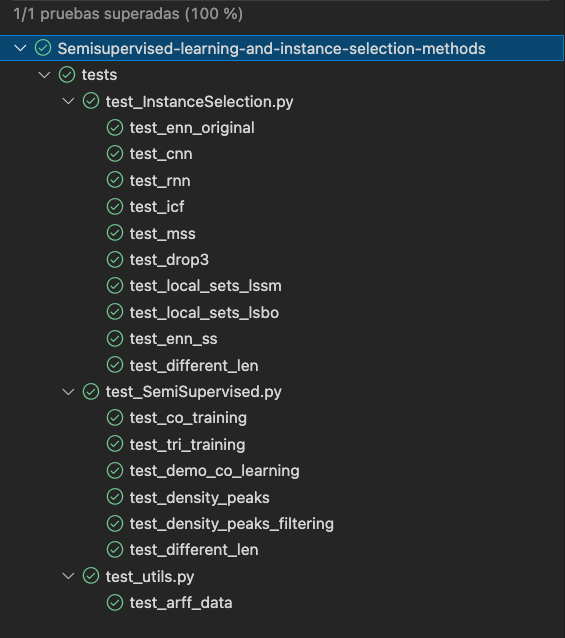
\includegraphics[width=0.5\textwidth]{../img/anexos/manual-programador/tests-superados-is-ssl}
\caption{Prueba base para algoritmos de aprendizaje semi-supervisado.}\label{fig:tests-superados-is-ssl}

\end{figure}

Además, se ha codificado una prueba para asegurar que se siguen leyendo los ficheros \texttt{ARFF} correctamente.

El resultado de las ejecuciones se puede ver la Figura~\ref{fig:tests-superados-is-ssl}.
















